\documentclass[../main.txt]{subfiles}

\begin{document}

\chapter{Overview of potential solutions}

This chapter theoretically elaborates on different approaches to implement the requirements defined in chapter \ref{requirements}.

\section{External encryption}
\label{sec:external_encryption}
An intuitive way of implementing a protocol that allows the exchange of logs among users is to rely on external encryption tools.
Suppose that Alice wants to share a log with Bob.
Alice could send the log to Bob with an encrypted email.
Emails can be encrypted with dedicated protocols, e.g. PGP~\footnote{Defined by IETF in \href{https://www.rfc-editor.org/rfc/rfc4880}{RFC4800}.} or S/MIME~\footnote{Defined by IETF in \href{https://www.rfc-editor.org/rfc/rfc8551.html}{RFC8551}.}.
Such encryption technologies allow Alice to confidentially share logs with others.
This approach, however, is limited and does not satisfy the identified requirements.
It is the responsibility of the user to correctly apply the protocol.
This is error-prone, it could lead to unintended security issues and it is not user-friendly.
Sharing the log with $n$ users requires Alice to send $n$ encrypted emails.
More importantly, this approach does not end-to-end encrypt logs because the server storing the logs still has access to the unencrypted data.
Since the Overseer server is not trusted, confidentiality is broken (security requirement S1).
Once an encrypted email is sent to the receiver there is no way for Alice to revoke any access to the log.
She loses control over the encrypted log because the email provider of Bob stores the cipher which is out of control of the toolchain.
This implies, that Alice can not revoke the access anymore (functional requirement F3).
Those limitations motivate the implementation of a more sophisticated protocol.

\section{Mutual encryption}
\label{sec:mutual_encryption}
The term mutual encryption refers to the idea that logs are encrypted mutually between users in the system.
If each user is assigned a key pair, a data owner can encrypt a log for each user separately.
The core idea is similar to the approach presented for external encryption (section \ref{sec:external_encryption}).
However, this approach integrates the encryption and decryption of logs into the toolchain.
To better understand this approach consider the following example.
A monitor component accesses data of Alice and therefore creates a log.
Since Alice needs to be able to access the log, the monitor encrypts the log under the public key of Alice and sends it to the server.
If Alice keeps her secret key private she is the only entity who can decrypt the log.
She can download the log, decrypt it, and also share it with Bob by re-encrypting it under the public key of Bob.
The re-encrypted data is then sent to the server where it is stored.
Bob can finally download and decrypt the shared log.

Alice can access the log because the monitor encrypted it with her public key.
She can also share logs with others.
The encrypted data is stored by the Overseer server.
This additionally allows Alice to request the deletion of the cipher from the server.
This way Alice can revoke the access to the log.
Thus, all functional requirements are fulfilled.
As long as all users have exclusive access to their secret key, this approach also ensures the confidentiality of the log (security requirement S1).
To defend against malicious data owners creating forged logs, the monitor component (e.g. the entity creating a log) needs to cryptographically sign the log before encryption.
If Alice shares the log, she does not share the plain log.
Rather, she encrypts the signed log.
Alice can not modify the existing log or create a completely new log because she is not able to compute a valid signature in the name of the monitor.
She could only succeed by knowing the secret key of the monitor.
This structure allows the receiver to verify if the log was created by a valid monitor component.
As a consequence, a forged log can be detected during decryption (security requirement S3).
Security requirement S2 can also be satisfied.
To achieve this, Alice does not only encrypt the signed log.
She additionally signs and includes the identity of the receiving user.
This allows receivers to verify if the log was intended for them.
Figure \ref{fig:mutual_encryption} shows the structure of a log before it is encrypted.
The actual access log is singed by the monitor.
The shared log is a data structure that contains the singed access log.
It additionally specifies the user with whom the log is shared with (e.g. receiver).
The shared log itself is signed by the data owner.
The signed share log is passed to the encryption algorithm.
After decryption a receiver can validate if the sender intentionally shared the log.
The receiver can also verify if the nested access log was singed by the claimed monitor.
\begin{figure}[t]
\centering
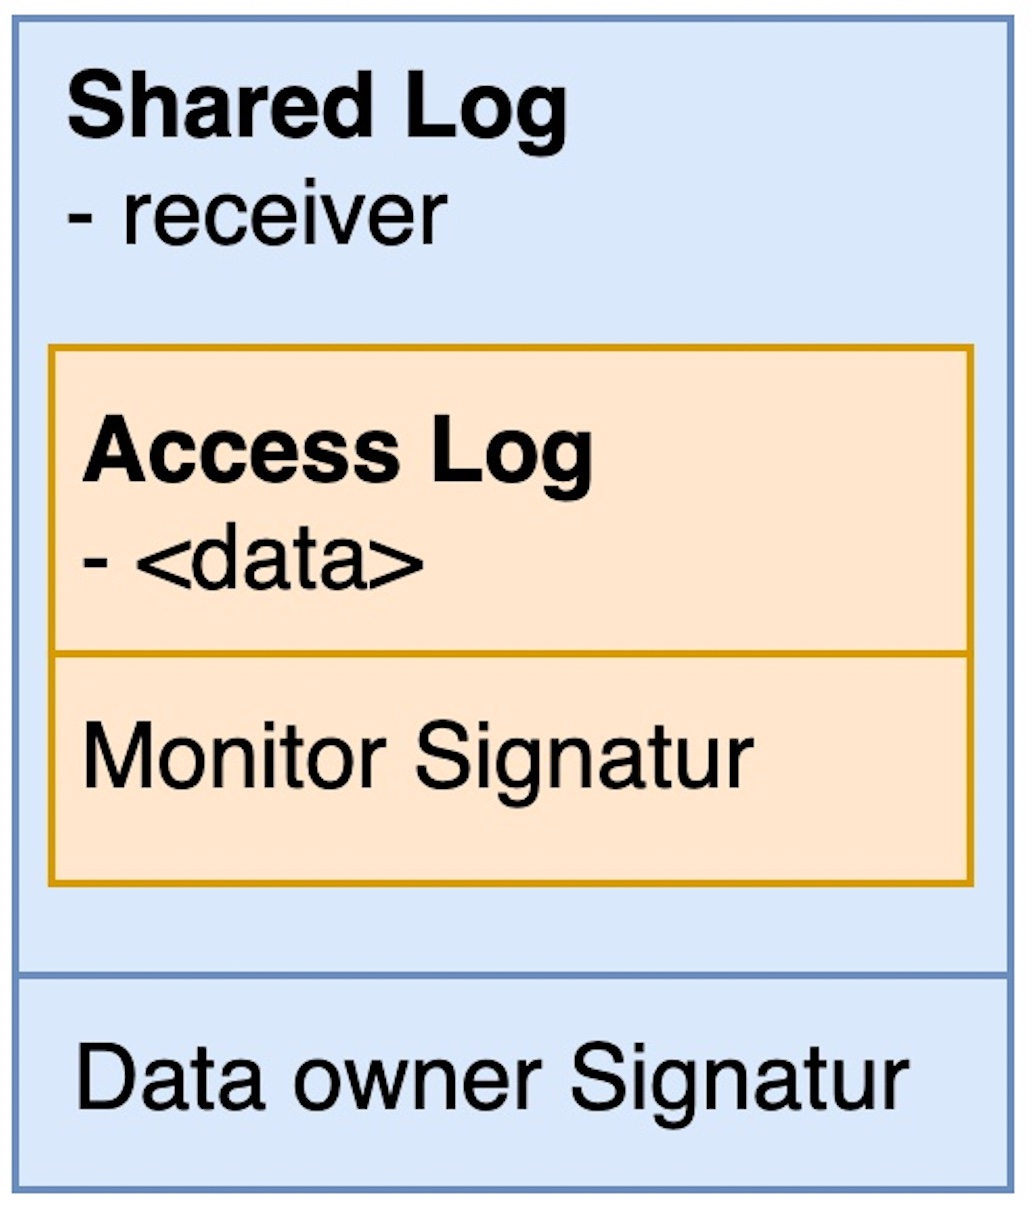
\includegraphics[scale=0.12]{../img/04/mutual_encryption.jpg}
\caption{Structure of a shared log before encryption.}
\label{fig:mutual_encryption}
\end{figure}
While this approach fulfills all functional and security requirements it suffers from performance problems.
Similar to external encryption, the whole log needs to be encrypted $n$ times if it is shared with $n$ users.
Much more problematic, however, is the application of asymmetric cryptography to application data.
Public-key cryptography relies on intense mathematical computations and should not be used to encrypt large amounts of data directly~\cite[340]{Eckert2018}.
Eckert justifies this with the fact that asymmetric encryption algorithms are muss less performant that symmetric algorithms.
Following her argumentation, asymmetric cryptography is therefore usually used to encrypt a symmetric key which finally encrypts the larger payload.
Thus, the implemented protocol should avoid the encryption of log data with asymmetric algorithms.


\section{Key server}
\label{sec:key_server}
The development of cloud computing and centralized software architectures motivated the idea of key servers~\cite{Seitz2003}.
A key server stores cryptographic keys on behalf of the user.
If a user authenticates against the server and has the required permissions it can access a particular key.
This can be useful in environments where multiple users need to access the same key.
The creator and owner of a key can upload the key to the key server.
If others require access to the key, the owner can modify the access policy.

The concept of a key server can also be applied to share encrypted logs.
Once a monitor creates a log because it accesses sensitive data of Alice, it creates a symmetric key and encrypts the log under this symmetric key.
The encrypted log is sent to the Overseer.
In order to decrypt the log, Alice requires access to this symmetric key.
Thus, the monitor needs to upload the generated key to the key server which allows Alice to download it.
If she wants to share the log with Bob, there is no need to re-encrypt any data in the Overseer.
Rather, she needs to tell the key server that Bob is allowed to access this key.
Alice can also revoke the access to the file.
She could simply tell the key server that a particular user is not allowed to access the key anymore.
However, if a malicious user stored the key on his local machine, the revocation does not have any effect.
It is better to additionally re-encrypt the encrypted log in the Overseer with a freshly generated key, which is then also uploaded to the key server.

This example shows that all functional requirements can be satisfied when utilizing a key server.
The techniques introduced in section \ref{sec:mutual_encryption} to satisfy security requirements S2 (sign the receiver of the shared log) and S3 (sign the access log) can be applied here, too.
Security requirement S1, however, can not be met because the administrator of the key server has access to all keys.
This allows him to potentially decrypt all logs which breaks confidentiality of the logs.
In section \ref{sec:end_to_end} it became clear that the encryption endpoints in E2EE systems can be defined quite arbitrary.
The here sketched protocol can nevertheless be classified as E2EE, if the key server is defined as valid decryption endpoint.
But it does not meet the intuitive understanding of E2EE.
The utilization of a key server also implies that we require an additional trusted component
This increases the attack surface of the system and does not adhere to the non-functional requirement N1 (minimal trusted entities). 







\section{Broadcast encryption}
\section{Hybrid encryption}

\section{Further investigations}


\todo{Consider ZOOM E2EE}
Zoom operates within a live environment, e.g. all participants are online. 
Encrypting data in Zoom relies on a DH key exchange during encryption. 
This implies, that each data packet is encrypted with its own key enabling forward secrecy. \cite{Isobe2021}

\todo{Consider E2EE in IM messaging Apps}
Our implementation should provide privacy but not anonymity, which is implemented in modern instant messaging applications~\cite{Akinbi2021}. 
IM applications usually decrypt each message with its own fresh key and provide PFS in some cases (e.g. Double Ratchet protocol)

\todo{E2EE content distribution/file sharing}
CloudSeal relies on Proxy Re-Encryption techniques.
CloudSeal does not implement a Web application, but relies on native (OS) to implement the crypto \cite{Xiong2012}.
The scheme proposed by \citeauthor{Hoerandner2020} also implements a Proxy Re-Encryption scheme. \cite{Hoerandner2020}
There are also bindings for WASM which implement Prox Re-Encryption (https://github.com/IronCoreLabs/recrypt-rs), thus one could implement Proxy Re-Encryption schemes also within web applications.
Problem: Proxy Re-Encryption requires a semi trusted server.
If the server has a re-encryption key, it can simply re-encrypt all traffic for this entity.
This fundamentally breaks E2EE.


\end{document}
